\chapter{Security}
This chapter describes the considerations and decisions taken to secure the back-end application.

\section{Authentication}
To make sure that malicious users can not abuse the back-end application, the decision to secure it through authentication was made. 
There was two options for how this could be handled. 

\subsection{The common approach}
This approach is to add a token of sorts to the header of the \gls{http} request. 
The downside of this option when working with \glsi{graphql} is that you can not add a \gls{http} header to your request in \glsi{graphiql} when you query from the browser, unless a browser extension for that specific thing is used. 
It would also not be very transparent or obvious when browsing \glsi{graphiql} that an authentication token is required for certain resources.

\subsection{The Facebook approach}
Facebook uses a root type called a \verb+viewer+ \citep{facebook:viewer}. 
The \verb+viewer+ represent the user making the requests. 
This can be used for several things. 
What we did was add a parameter on the root type \verb+viewer+ so that the \verb+viewer+ takes a token. 
This approach makes it very obvious that the \verb+viewer+ 'area' is restricted and requires a authentication token to access. 
Every resource that requires an authenticated user will then be underneath the \verb+viewer+ type and every other endpoint are exposed outside the \verb+viewer+ object. 
On figure \ref{fig:queryViewer} this is illustrated.

\graphic{0.6}{query}{\gls{api} documentation for the root query with the viewer and login queries returning the viewer type}{fig:queryViewer}

Notice that both of them returns a \verb+viewer+ type. 
When logging in, the same \verb+viewer+ as you can get when asking for the \verb+viewer+ with your token, is returned. 
This is to save a round-trip after logging on, figure \ref{fig:loginSequence2}. 
Another approach is to \verb+login+ and only receive a token which can then be use to query for the \verb+viewer+. 
But that approach is slower since it requires two round-trips as shown on figure \ref{fig:loginSequence1}.

\begin{figure}
    \centering
    \begin{subfigure}[b]{0.45\textwidth}
        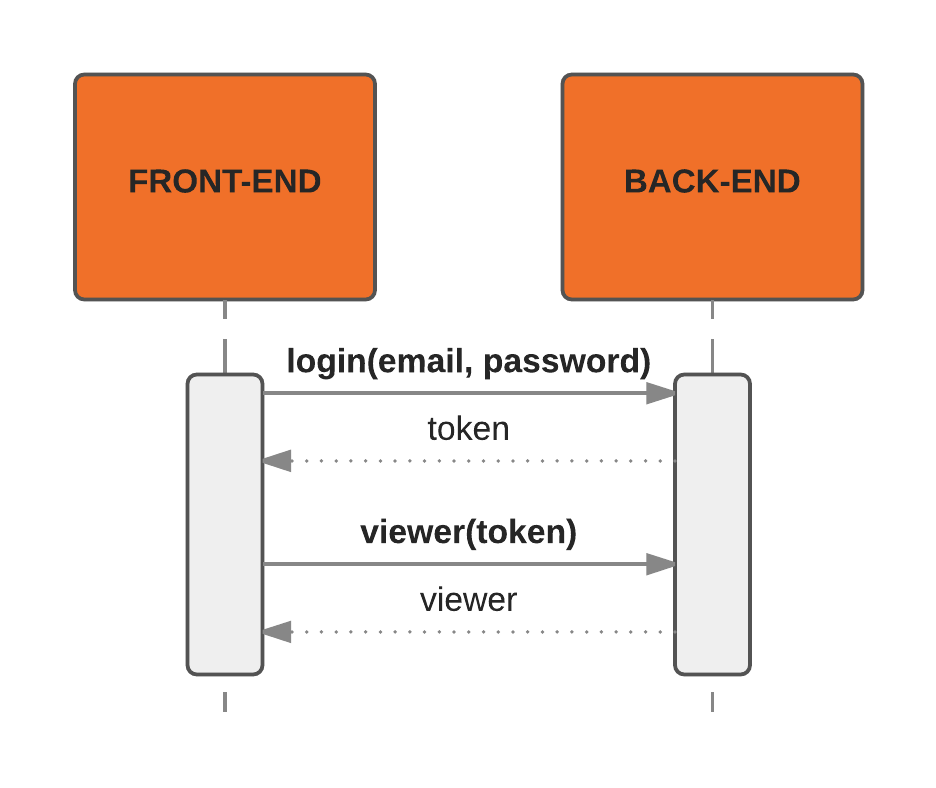
\includegraphics[width=\textwidth]{graphics/loginSequence1}
        \caption{Login returns token to further query with}
        \label{fig:loginSequence1}
    \end{subfigure}
    \hfill
    \begin{subfigure}[b]{0.45\textwidth}
        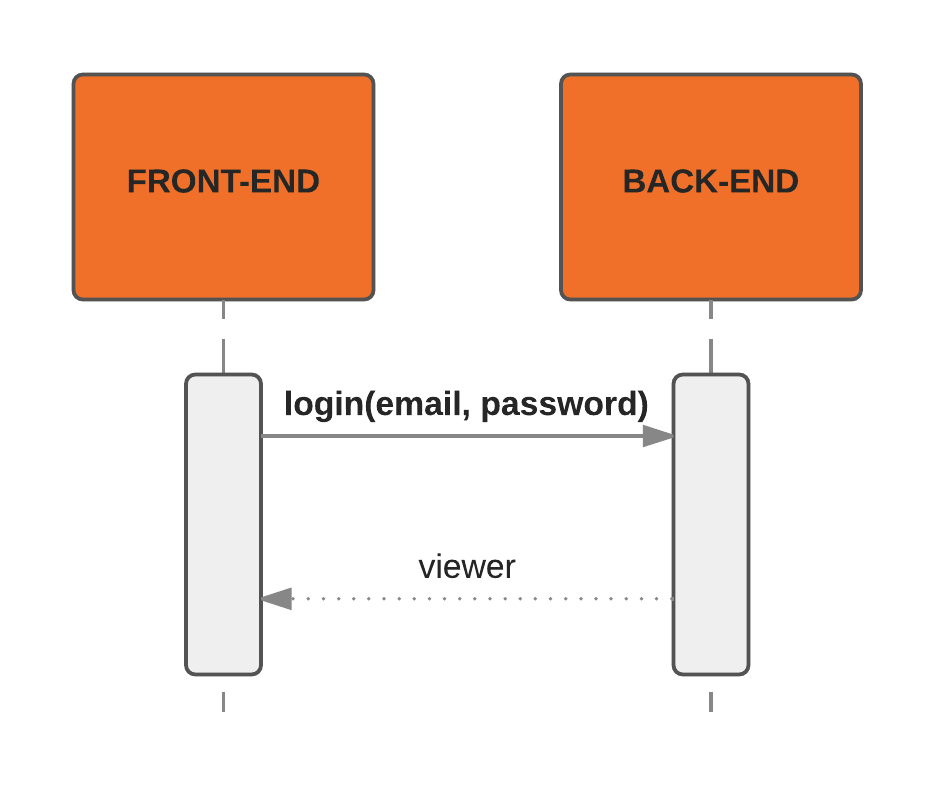
\includegraphics[width=\textwidth]{graphics/loginSequence2}
        \caption{Login returns viewer for direct access}
        \label{fig:loginSequence2}
    \end{subfigure}
    \caption{Authentication token request flows}
\end{figure}

The most important queries to get behind authentication is the mutations since they are the queries that manipulate data. 
So all the mutations are hidden behind a \verb+MutationViewer+. 
This is shown on figure \ref{fig:mutationViewer}. 
When passing the token to the viewer, it is checked in the database and the user owning the token, if any, is then passed down the graph so that the queries below the viewer know exactly who the user is. 

\graphic{0.6}{mutation}{\gls{api} documentation for the MutationViewer type}{fig:mutationViewer}

\subsection{Token generation}
The token is generated on login and removed on logout. 
An \glsi{npm} package named \verb+node-uuid+ is used to generate an RFC4122 v4 \gls{uuid}, which is then stored with the user. 

The odds of creating duplicate tokens when using RFC4122 v4 is extremely small. 
On average it would take a few trillions of \gls{uuid}s to generate two duplicate tokens \citep{authentication:uuid}.
